%!TEX root = ./Structure_rapport_final.tex


% Resitue le sujet dans une problématique générale ;
%  -restitue le sujet dans un cadre de gestion plus global
% - doit également justifier le bien-fondé de l’étude en fonction des demandes
% • Donne les objectifs qui ont été fixés pour répondre à la question posée ;
% • Présente la démarche qui va permettre de répondre aux objectifs.


% \subsection{Présentation des milieux marins profonds}
% - milieu peu connu, écosystème particulier --> communauté sur laquelle on travaille 
% - particuliarité des canyons 
% - Rôle de ces espèces dans les chaines trophiques (plus faibles maillons et MM/oiseaux)
% - communauté de poisson méso-bathy pélagiques 

% \subsubsection*{Présentation de l'environnement}
The deep ocean is the largest marine habitat of Earth, and represents 95\% of ocean's volume \citep{danovaro2017,salazar2016,webb2010}. From a biology perspective, deep-sea encompasses everything beneath euphotic (or epipelagial) zone, where the solar radiations are too low and precludes photosynthesis \citep{baker2020,danovaro2017,salazar2016} (Figure~\ref{fig:dsl}). Between 200 to 1000m deep (mesopelagic zone), light fades and temperature decreases, because solar luminance is absorbed exponentially in upper sea layers \citep{reynolds2001}. From 1000 to 4000m deep (bathypelagic zone), no sunlight remains and the habitat is pitch-black; salinity and temperature are stable (between -1.8 to 2°C), and pressure keeps on increasing by 1 atm every 10m \citep{danovaro2017}. 

\begin{figure} [!htbp]
	\begin{center}
		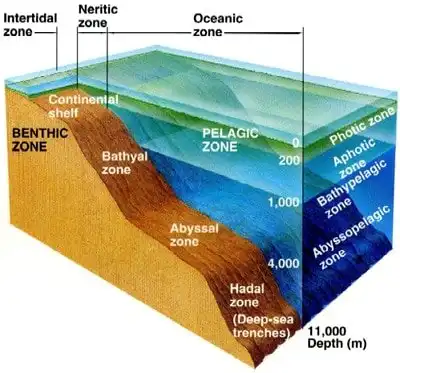
\includegraphics[width=0.5\textwidth]{sea_layers.png}
	\end{center}
	\caption[Sea layers]{Sea layers along depth, from The MarineBio Conservation Society (\url{https://www.marinebio.org/oceans/deep-sea/}).}
	\label{fig:dsl}
\end{figure}

Despite these extreme conditions, deep-sea is far from being lifeless. In fact, deep-sea is considered to be the largest biome of the Earth, and contains 70\% of ocean's microbial cells and 60\% of its heterotrophic activity, playing a crucial role in biogeochemical cycles \citep{salazar2016}. Studies from \citet{grassle1992,parkes1994,todo2005} shown that life could be found everywhere in the deep-sea, with remarkably high and stable diversity. Moreover, these very particular conditions have resulted in a high specialization of the inhabiting fauna, with species that are absent from shallower waters \citep{garcia2021}. With first studies launched in the 60's, less that 0.0001\% of the area has been investigated so far and this habitat remains understudied \citep{danovaro2017,richards2019}. Thus, deep-sea remains the most unknown biome of the planet with estimated 10 million species that are yet to discover \citep{danovaro2017,grassle1992}. In particular, data are lacking to evaluate the impact of climate change on the biodiversity of the largest reservoir of biomass, mainly because exploring deep-sea is difficult and requires specific tools, such as rovers \citep{danovaro2008,danovaro2014}. Firstly, deep-sea were regarded as a ore reservoir of its soil, where manganese and other metal deposits could be found and extracted, or even as a dumping site for nuclear wastes \citep{baker2020,gillet2013,halfar2002}. But since past decades, capacity of exploration of the deep-sea expanded spectacularly, allowing to discover more about the deep-sea ecosystems\citep{danovaro2014}.

In particular, continental margins, which separates continental shelf from abyssal plains are investigated, because their heterogeneous topography implies varied habitats and hydrodynamics, with impacts on the whole food webs \citep{danovaro2009,fernandez-arcaya2017}. Along continental margins, deep-sea canyons, that incises the edges of continental shelf, appears to be ``biodiversity hotspots'' for pelagic life, in terms of diversity and abundance \citep{aissi2012,danovaro2009,gillet2013,robertson2020}. Caynons are also reported having a high level of endemism \citep{danovaro2009,danovaro2017}. 

Because they have a crucial role in transferring organic matter and sediments from rich and productive shallow shelf to the low-nutrients deep-sea, canyons constitute peculiar habitats, with evidences of an important biomass and diversity inside and around them \citep{canals2006,danovaro2009,deleo2012,sion2019,stefanescu1994}. Indeed, canyons have higher nutrients concentrations than in adjacent areas, due to down-welling currents creating a funnel-effect \citep{fernandez-arcaya2017}. Thus, primary production is enhanced, and makes canyons favorable habitats for filters and suspension feeders \citep{fernandez-arcaya2017,sion2019}, but also for low to medium trophic levels organisms, such as euphausiids, shrimps, squids and meso- and bathypelagic fishes \citep{aissi2012,gaskett2001,pusch2004}. Abundance of nutrients and preys attracts top predators (cetacean, sharks, large pelagic), some of them being only encountered in these habitats \citep{aissi2012}. Finally, canyons provides many ecological services and play a role in sustaining deep-sea food webs through the transport of nutrients, providing habitat for nursery and refuges \citep{fernandez-arcaya2017}. \citet{company2008} suggests that by these services, canyons enhance recruitment of commercialized species, and thus, may mitigate the effect of their overexploitation. Therefore, canyons can be described as ``keystone structures'', as an interface between productive continental shelf and deep-sea, with evidence of their benefits and supports for fisheries \citep{company2012,fernandez-arcaya2017}.

% \subsubsection*{Présentation des poissons méso et bathy pelagiques}
Meso- and bathypelagic fishes are found abundantly in every ocean, except Arctic, and are the dominant zooplankton consumers in most oceans, playing a key role in trophic networks \citep{davison2015,salvanes2009}. Living between 200-1000m (mesopelagic) and over 1000m (bathypelagic) deep, these deep-sea fishes displays very high biomass, estimated to be around ten billion tonnes in total \citep{garcia2021,gjoesaeter1980,richards2019}. Though, abundance of these fishes varies along depth and daytime, because most of them perform vertical diel migration to feed on shallower depth during night, and abundance's estimation can be biased by sampling time \citep{catul2011,gaskett2001,garcia2021,pusch2004,salvanes2009}. Performing migrations, meso- and bathypelagic fishes ensure biogeochemical cycling through respiration and excretion but also when predated by carnivorous \citep{garcia2021,spitz2019}. Because of their ubiquity, their biomass and the high efficiency of energy transfer from phytoplankton (respiring 10\% of the primary production), meso- and bathypelagic fish play an important part of the biological pump \citep{garcia2021,spitz2019}.

Meso- and bathypelagic fish can show adaptations to their environment such as highly sensitive eyes, dark body and ventral light organs (photophores) to match their low-light habitat and reduced metabolic rates to lower oxygen consumption in poorly oxygenated waters \citep{salvanes2009,farre2016}. Photophores have a role in camouflage, foraging, courtship behavior, with different patterns between males and females. They are also species specific which helps identification \citep{paitio2020,salvanes2009}. Finally, depth and associated pressure play a role in the morphology of deep-sea fishes, which tend to have more elongated body with increasing depth, while manifesting an enlargement of the anterior body that increase gill surface and the ability to capture oxygen \citep{farre2016}. Most of the life history traits of meso- and bathypelagic fish remains unknown and needs to be further investigated, with relatively poor and non consistent literature \citep{childress1980,salvanes2009}. The mesopelagic communities are dominated by Myctophidae family, in terms of abundance, diversity and biomass, and represents at least 20\% of the whole oceanic ichthyofauna \citep{catul2011,kozlov1995,pusch2004}.

% \subsubsection*{Zoom sur le gdG}

Several studies focused on exploring deep-sea fish diversity near seamounts, mid-ocean ridges or in abyssal depths \citep{cook2013,sutton2013}, but very little is known about meso- and bathypelagic species inhabiting deep-sea canyons \citep{kenchington2020}. Nevertheless, given the essential role of the oceanic pelagic fish community in food webs, linking the epipelagic organic matter to top predators, requires a better knowledge of species constituting this fundamental compartment \citep{davison2015,gaskett2001}. Furthermore, considering how important canyons are for fisheries and carbon sequestration, knowing more about the communities inhabiting them is crucial to ensure sustainability of ecosystems and provided services, through marine management and conservation \citep{fernandez-arcaya2017,vandenbeld2017a}.

Located in the temperate North-east Atlantic Ocean, the Bay of Biscay's continental shelf is highly productive, with nearly 700 fish species and 35\% of the world total marine mammals identified in this region \citep{borja2019}. This productivity relies on heavy rivers discharge and strong influence of eastward winds, tides and eddies \citep{borja2019,akpinar2020}. Thus, plankton, benthic and pelagic communities have been widely studied for several decades, with some fish communities being annualy monitored \citep{borja2019,doray2018}. Conversely, there is little knowledge on canyon, abyssal and bathyal communities in this area \citep{borja2019}. The continental slope of the Bay of Biscay divides in two the of France's Atlantic EEZ (Exclusive Economic Zone) and is incised by about 135 canyons \citep{bourillet2006,spitz2019,vandenbeld2017} (Figure~\ref{fig:bbm}). If proven to be rich in cold-water coral reefs, the largest part or the area remains poorly explored, especially deep-pelagic communities \citep{garcia2021,vandenbeld2017a,webb2010}. In consequence, the similarity or differences within species inhabiting these ecosystems are unknown \citep{kenchington2020}. 

\begin{figure} [!htbp]
	\begin{center}
		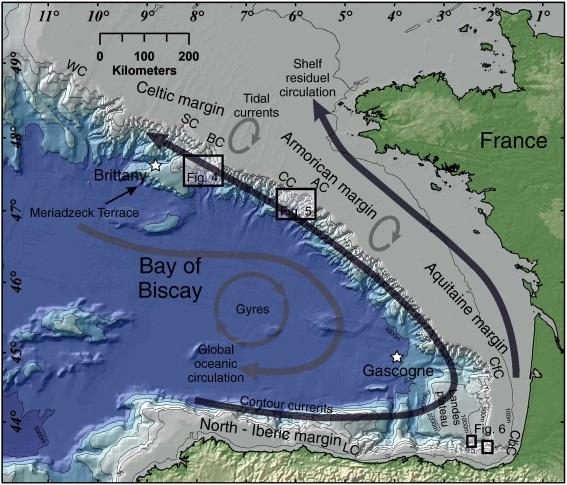
\includegraphics[width=0.6\textwidth]{Biscay_Bay_map.png}
	\end{center}
	\caption[Map of the studied area]{Location of the studied area, from \citep{bearez2017}.}
	\label{fig:bbm}
\end{figure}

One way to characterize an ecosystem is to look at the factors that control biodiversity patterns and to identify the key functions provided by this ecosystem \citep{aneeshkumar2017,brindamour2011,farre2016}. Functional diversity, which is the value and range of functional traits displayed by the organisms of a given ecosystem, can inform on ecosystems functioning and about their resilience facing a change in the environment \citep{dumay2004,martini2020}. Moreover, the use of functional traits to characterize functional niches of species highlights some competition or adaptation processes within a communtinity of an ecosystem \citep{aneeshkumar2017}. Indeed, comparison of functional niches is an effective way of assessing ecological similarity of species, based on the way they share, or not, certain morphological, behavioral or physiological characteristics \citep{aneeshkumar2017,farre2016,winemiller1991}.

This approach seems particularly well suited to study fish communities, because morphological traits are considered being good indicators of ecological habits of species, indicating how species use available resources \citep{farre2016,winemiller1991}. Successfully applied for freshwater ecosystems and marine coastal environments, this approach has not been much used on deep-sea communities where functional traits shaping ecological niches remains mostly unknown \citep{aneeshkumar2017,farre2016}. Conditions become more extreme and the food availability decreases with depth, so deep-sea are often thought to be poor in terms of functional diversity \citep{aneeshkumar2017,mason2008,novotny2018}. This would mean that most (if not all) deep-sea species are generalists, and suggests that competition is highly probable to access the little food available .

Because species displaying the same functional niche can be considered as part of the same functional group, our hypothesis is that species occupying similar functional niches insure redundant function within an ecosystem and be in competition, whereas species displaying very different functional niches would be segregated. Hence, the aim of this work is to assess functional diversity of deep-sea canyons fish of the Bay of Biscay, which, for the moment, is barely known \citep{kenchington2020}. Using functional traits to assess functional niches of species, our main objectives are (i) to characterize functional diversity of most-abundant canyon species, (ii) to measure the range and degree of overlap of functional niches and (iii) to identify the traits that structure the most these communities.

% \subsection{Axes pour une meilleure connaissance de ces écosystèmes}
% - comment les espèces se partagent les ressources (bcp d'études déjà terrestres)
%          --> focus sur cette communauté particulière qui est pour l'instant peu connue

% - 2 approches possibles: 
% 		- espèce-centrée : seule ou en compétition --> mais limitant pour la comparaison entre écosystèmes différents. 
% 		- communautaire : certaines espèces sont-elles redondantes ? Plusieurs espèces
% occupent la même niche en cas de chevauchement, occupent la même niche fonctionnelle. Se focaliser
% sur les fonctions plutôt que sur l'espèce. --> Permet une généralisation de la méthode et une comparaison entre écosystèmes
% 		- Individus appartenant à la meme niche peuvent être considérés comme appartenant
% à la même boîte fonctionelle. 
% ==> Caractériser un écosystème par les fonctions qu'ils présentent plutôt que par ses espèces

% \subsection{Présentation de la démarche et des objectifs}
% - mieux connaitre ces communautés à travers les niches qu'elles occupent dans les écosystèmes
% - caractériser leurs niches trophiques, comportements, habitats, sensibilité des espèces, 
% particularité des espèces, voir les avantages de partager les niches 
% - Envisager une approche universelle, permettant la comparaison d'écosystèmes

% - Hypothèses: chevauchement de niches entre les espèces, entrainant de la compétition entre les espèces ayant des fonctions similaires, ou ségrégation, où les espèces
% utilisent des ressources distinctes et ont des fonctions différentes

